%
% teil1.tex -- Beispiel-File für das Paper
%
% (c) 2020 Prof Dr Andreas Müller, Hochschule Rapperswil
%
% !TEX root = ../../buch.tex
% !TEX encoding = UTF-8
%
\section{Mathematische Grundlagen
\label{wavelets:section:teil1}}
\rhead{Problemstellung}

\subsection{Diskrete Fouriertransformation (DFT)
\label{wavelets:subsection:DFT}}
Um die CWT richtig nachvollziehen zu können lohnt es sich vorab mit dem Modell der diskreten Fourier Transformation (DFT)

\begin{equation}
	X(k)=\frac{1}{N}\sum_{n=0}^{N-1}x(n)\cdot e^{-j\frac{2\pi}{N}\cdot k\cdot n}
	\label{wavelets:equation1}
\end{equation}
auseinanderzusetzen. Hierbei beschreibt $X(k)$  das Fourier-transformierte Signal in Abhängigkeit der Frequenz $k$.
Die Funktionsweise lässt sich aus der Gleichung direkt ableiten.
Ein Signal $x(n)$ wird an jeder diskreten Stelle $x(n)$, wobei $n$ die ganze Zahlen von $0$ bis $N-1$ durchläuft, mit der Exponentialfunktion \[e^{-j\frac{2\pi}{N}\cdot k\cdot n}\] verrechnet.

Die Exponentialfunktion kann auch mit

\begin{equation}
	\cos \left( \frac{2\pi}{N}kn \right) -j\cdot \sin \left( \frac{2\pi}{N}kn \right)
	\label{wavelets:equation2}
\end{equation} 
beschrieben werden. Das Minuszeichen bestimmt nur den Umlaufsinn des komplexen Einheitsvektors im Einheitskreis.
Es wird also ein Signal an jeder Stelle $x(n)$ mit der komplexen Exponentialfunktion für die betrachtete Frequenz $k$ verrechnet und das über alle Punkte $x(n)$ für $n=0,1,2,...N$. Die resultierende Summe wird dann über die Anzahl verrechneter Punkte geteilt, was dem arithmetischen Mittelwert entspricht.

\begin{figure}
	\centering
	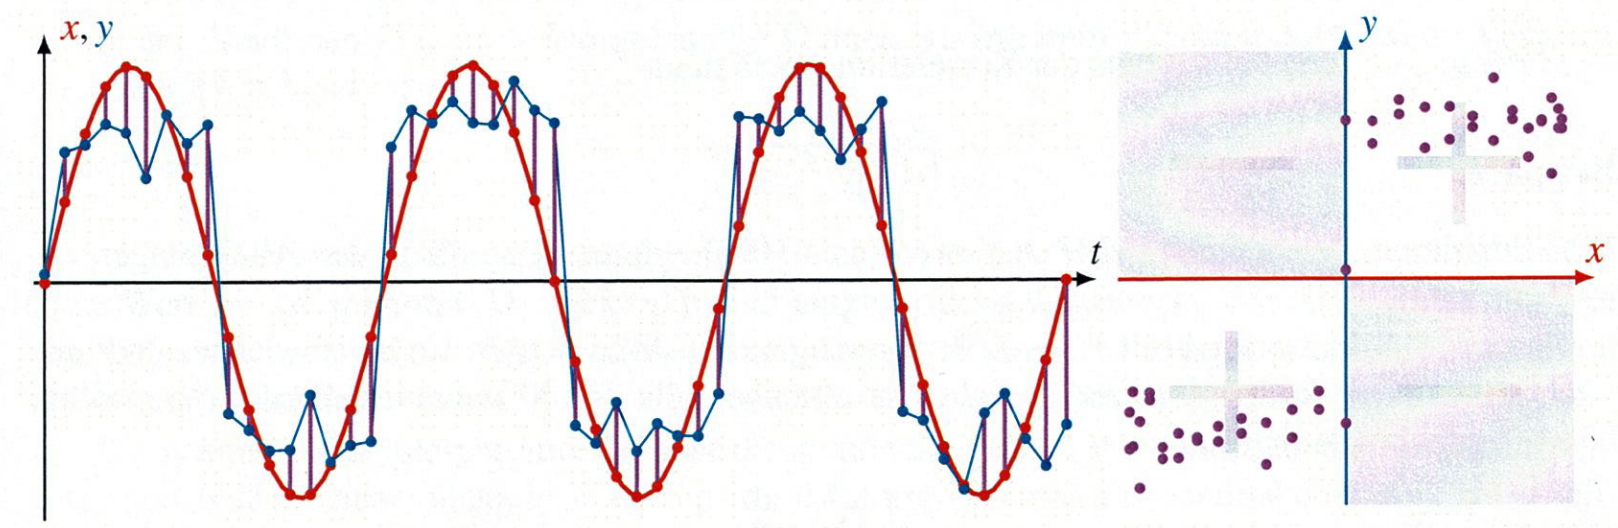
\includegraphics[width=0.49\textwidth]{papers/wavelets/images/2_DFT1.png}
	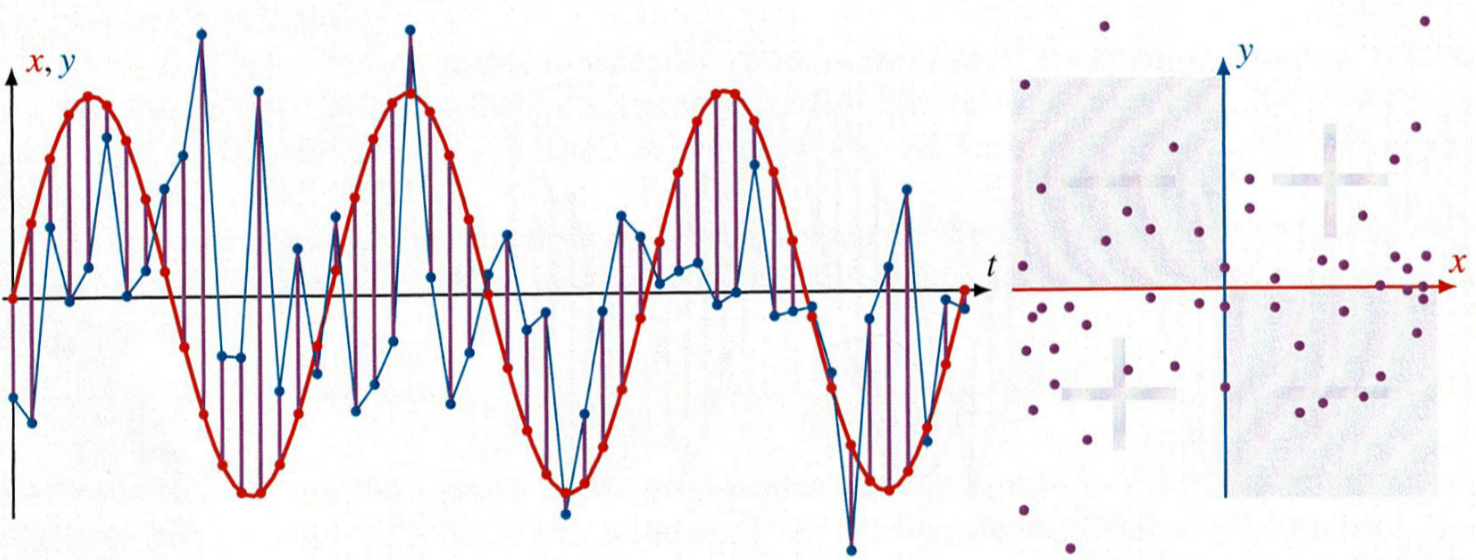
\includegraphics[width=0.49\textwidth]{papers/wavelets/images/2_DFT2.png}
	\caption{Darstellung zur Funktionsweise der DFT. In der linken Hälfte mit einer hohen Deckung zwischen Signal (blau) und der gesuchten Sinusfrequenz $k$ (rot). In der rechten Hälfte ein zufallsverteiltes Signal mit schlechter Überdeckung. Die Deckung wird nebenan in einem $+$ \& $-$ Verrechnungsplot, der aus vier Quadranten besteht, ausgegeben.}
	\label{wavelet:fig:2_DFT1&2}
\end{figure}

\begin{figure}
	\centering
	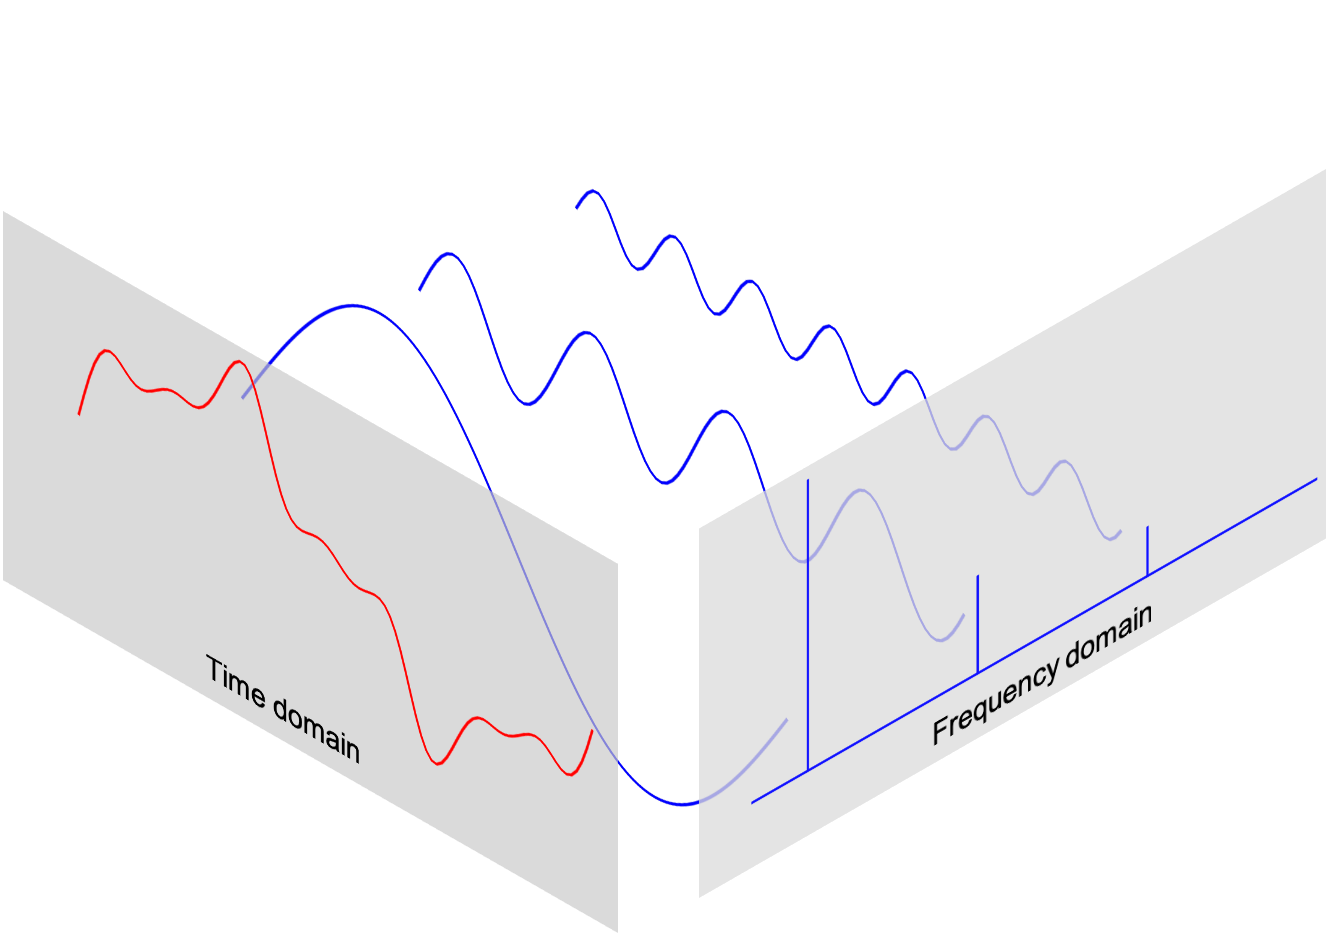
\includegraphics[width=0.5\textwidth]{papers/wavelets/images/3_AmplitudengangExtraktionDFT.png}
	\caption{Erzeugung des Amplitudenganges bei der DFT. Extraktion der vorhandenen Sinusanteile (blau) aus dem Zeitsignal (rot) }
	\label{wavelet:fig:AmplitudengangExtraktionDFT}
\end{figure}

Anstelle der Funktion \ref{wavelets:equation2} kann man sich im 2D vereinfacht die Verrechnung des Wertes $x(n)$ an der Position $n$ mit dem $\sin(\frac{2\pi}{N}kn+\phi)$ vorstellen, wobei $\phi$ die Phasenverschiebung des Sinuses beschreibt. Das $\phi$  wird in der Formulierung \ref{wavelets:equation2} mit dem Cosinusanteil miteinbezogen. Wenn nun das Signal den Sinus mit der Frequenz $k$ enthält wie in Abbildung \ref{wavelet:fig:2_DFT1&2}, kommt es zu einer Überdeckung und entsprechend hoher Aufsummierung. Das kann in der linken Hälfte der Abbildung \ref{wavelet:fig:2_DFT1&2} an den Verrechnungspunkten die alle in den positiven Quadranten liegen nachvollzogen werden. In diesem Fall kommt es zu einem Amplitudenausschlag auf der entsprechenden Frequenz. In Abbildung \ref{wavelet:fig:AmplitudengangExtraktionDFT} ist das schematische für ein Signal (rot) und die enthaltenen Sinusanteile (blau) dargestellt. Die Frequenzdomäne entspricht dabei dem Bildbereich des transformierten Zeitsignals (rot). Im Gegensatz dazu werden andere Frequenzanteile oder zufallsverteilte Signalpunkte durch den ständigen Wechsel von plus und minus in der Summe gegen Null gehen, was in der rechten Hälfte von Abbildung \ref{wavelet:fig:2_DFT1&2} eher der Fall ist. Die Verrechnungspunkte liegen nun verstreuter in den plus und minus Quadranten. Mit diesem Prinzip kann die DFT die Frequenzanteile ermitteln (Abbildung \ref{wavelet:fig:2_DFT1&2} \& \ref{wavelet:fig:AmplitudengangExtraktionDFT}).

An der Stelle soll noch der Link zwischen Frequenzspektrum (Autospektrum) und Frequenzgang (englisch Frequency Response Function FRF) gemacht werden.

\begin{itemize}
	\item Beim Autospektrum handelt es sich lediglich um die Fouriertransformierte eines Signales, meistens des Ausgangssignals.
	\item Der Frequenzgang ist die Übertragungsfunktion zwischen Eingang und Ausgang. Dabei wird der Quotient aus der Fouriertransformierten des Ausgang $Y$ über dem ebenfalls transformierten Eingang $X$, \[\frac{FFT(Y)}{FFT(X)} = FRF,\] gebildet.
	Dieses Verhältnis von Antwort zu Erregung lässt eine eindeutige Bestimmung der Resonanzen und des Phasenverlaufes zu.
\end{itemize}

\begin{figure}
	\centering
	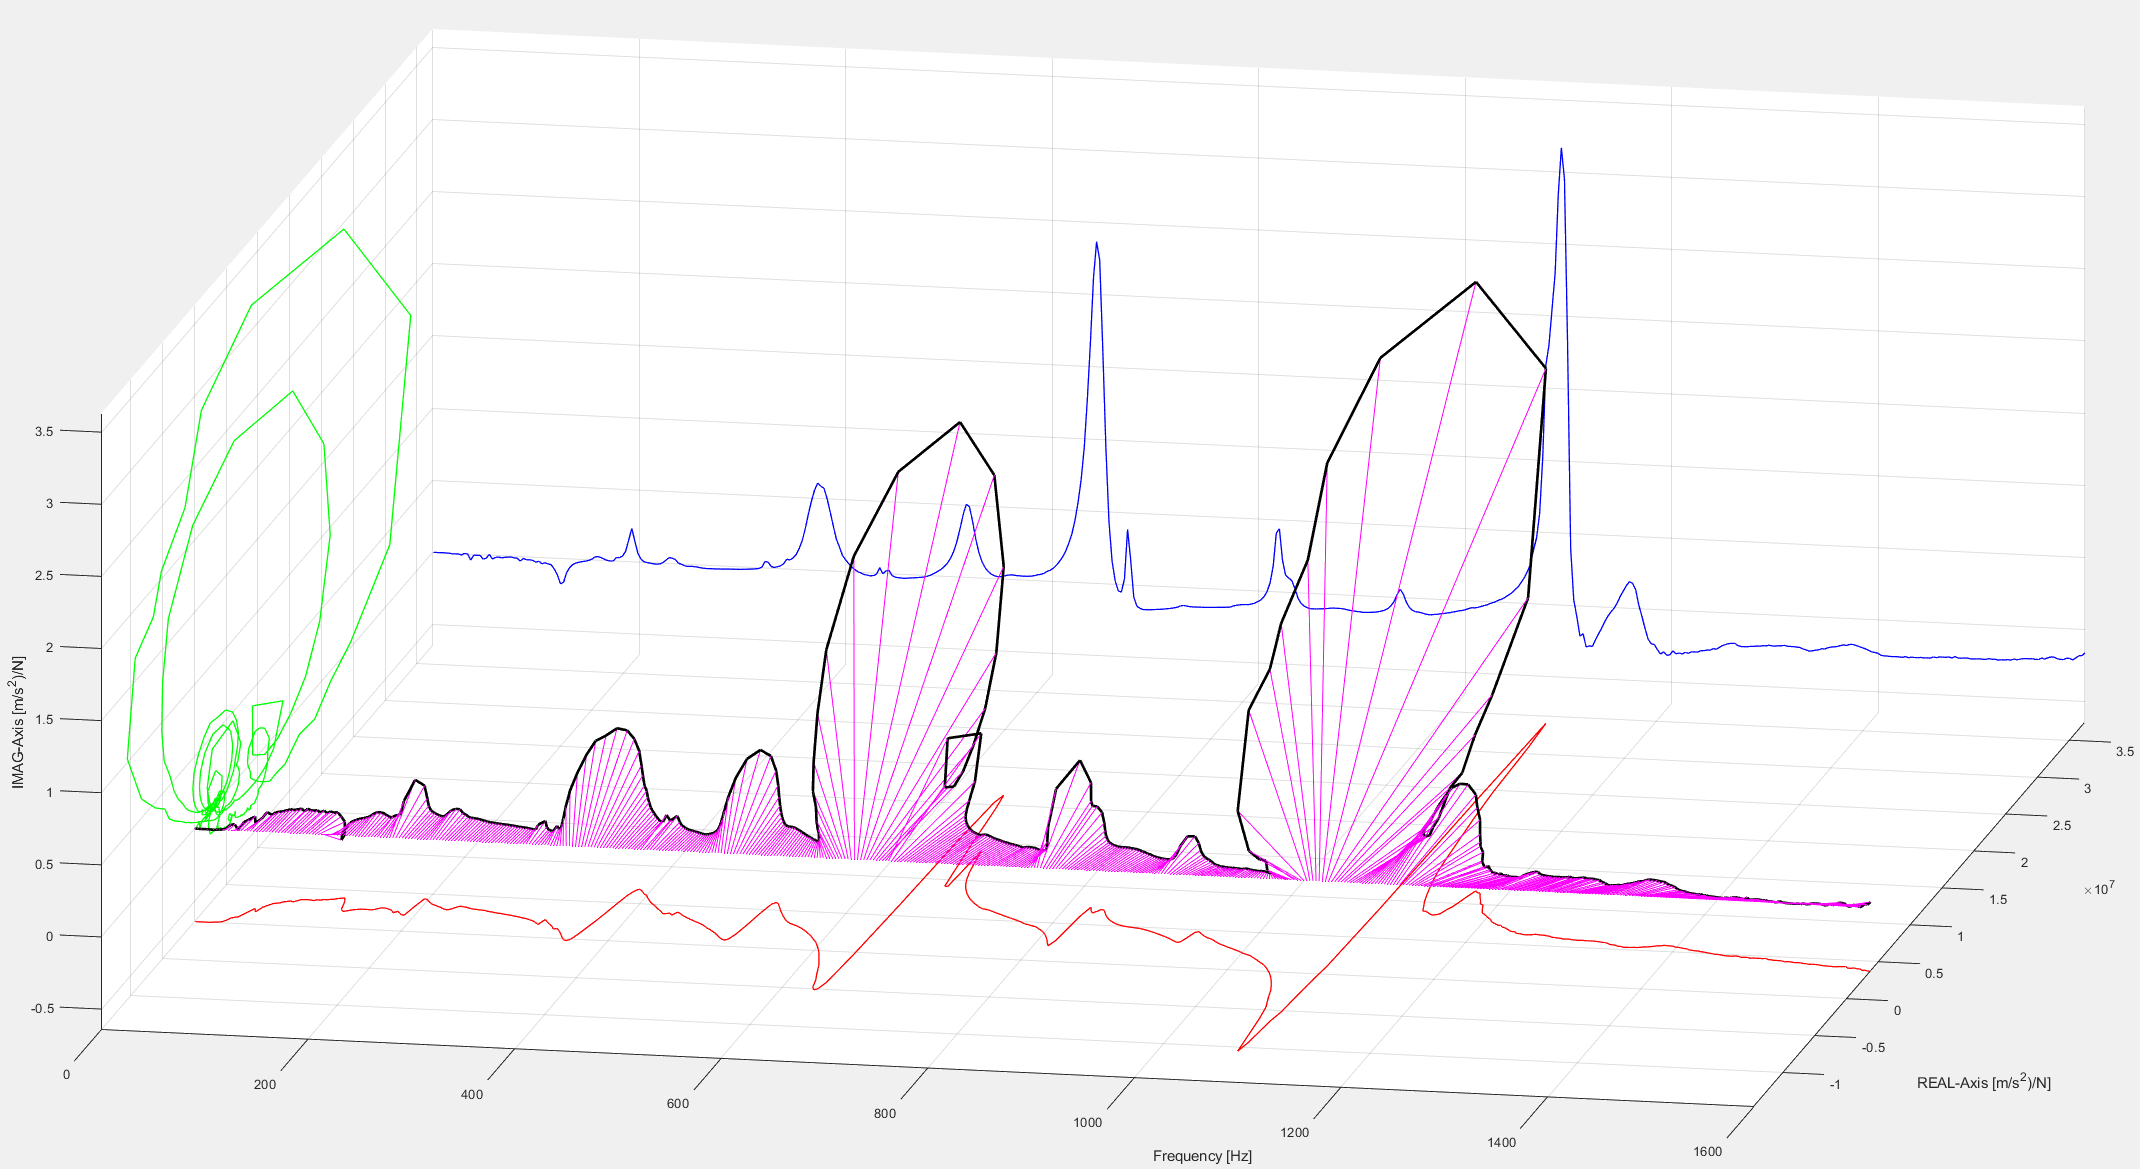
\includegraphics[width=\textwidth]{papers/wavelets/images/4_FRF_iso.png}
	\caption{3D-Darstellung eines Frequenzganges aus einem gemessenen Eingang (Shakersignal) und Antwort (Piezo-Sensor an einer Struktur).}
	\label{wavelet:fig:FRF_iso}
\end{figure}

Die 3D-Abbildung\ref{wavelet:fig:FRF_iso} zeigt einen FRF und die Projektionen in seine Bestandteile.

\begin{itemize}
	\item Der Realteil entspricht dem auf die reele Ebene abgebildete Projektion des FRF. Der Realteil geht in der Resonanz auf Null, d.h. alle Energie liegt im Imaginärteil. Ausserdem kann die Resonanz am vorhanden Phasensprung im Realteil abgelesen werden.
	\item Der Imaginärteil des FRF ist analog die Projektion auf die imaginäre Ebene , hier lassen sich eindeutig die Resonanzfrequenzen auslesen. Das System ist in Resonanz, zur Phase der Anregung, um 90° Phasenverschoben.
	\item Die Ortskurve ist die auf den Einheitskreis abgebildete Projektion des FRF. Anhand der Ortskurve kann der Verlauf der Phase nachvollzogen werden.
\end{itemize}

\subsection{Kontinuierliche Wavelettransformation (CWT) anhand des Morlet Wavelet
	\label{wavelets:subsection:CWT}}
Die stetige Wavelettransformation (CWT) eines Signals $f(t)$ ist

\begin{equation}
	W_{a,b}=\langle f \; , \; \psi_{a,b} \rangle = \frac{1}{\sqrt{a}}\int_{-\infty}^{\infty} f(t)\cdot\psi\left(\frac{t-b}{a}\right) dt,
	\label{wavelets:equation3}
\end{equation}
wobei
\[\psi_{a,b}(t)=\psi\left(\frac{t-b}{a}\right)\]
definiert wird. Was sofort auffällt ist, dass man nun zwei unabhängige Variablen besitzt. Zum einen ist das die Frequenzskalierung $a$, so genannt weil mit diesem Faktor das Mutterwavelet gedehnt oder komprimiert wird, man somit die Frequenz des Wavelets festgelegt. Zum anderen die Verschiebung auf der Zeitachse $b$, also wo das Wavelet sich zeitlich befindet (Abbildung \ref{wavelet:fig:5_WaveletKompUndShift}).

\begin{figure}
	\centering
	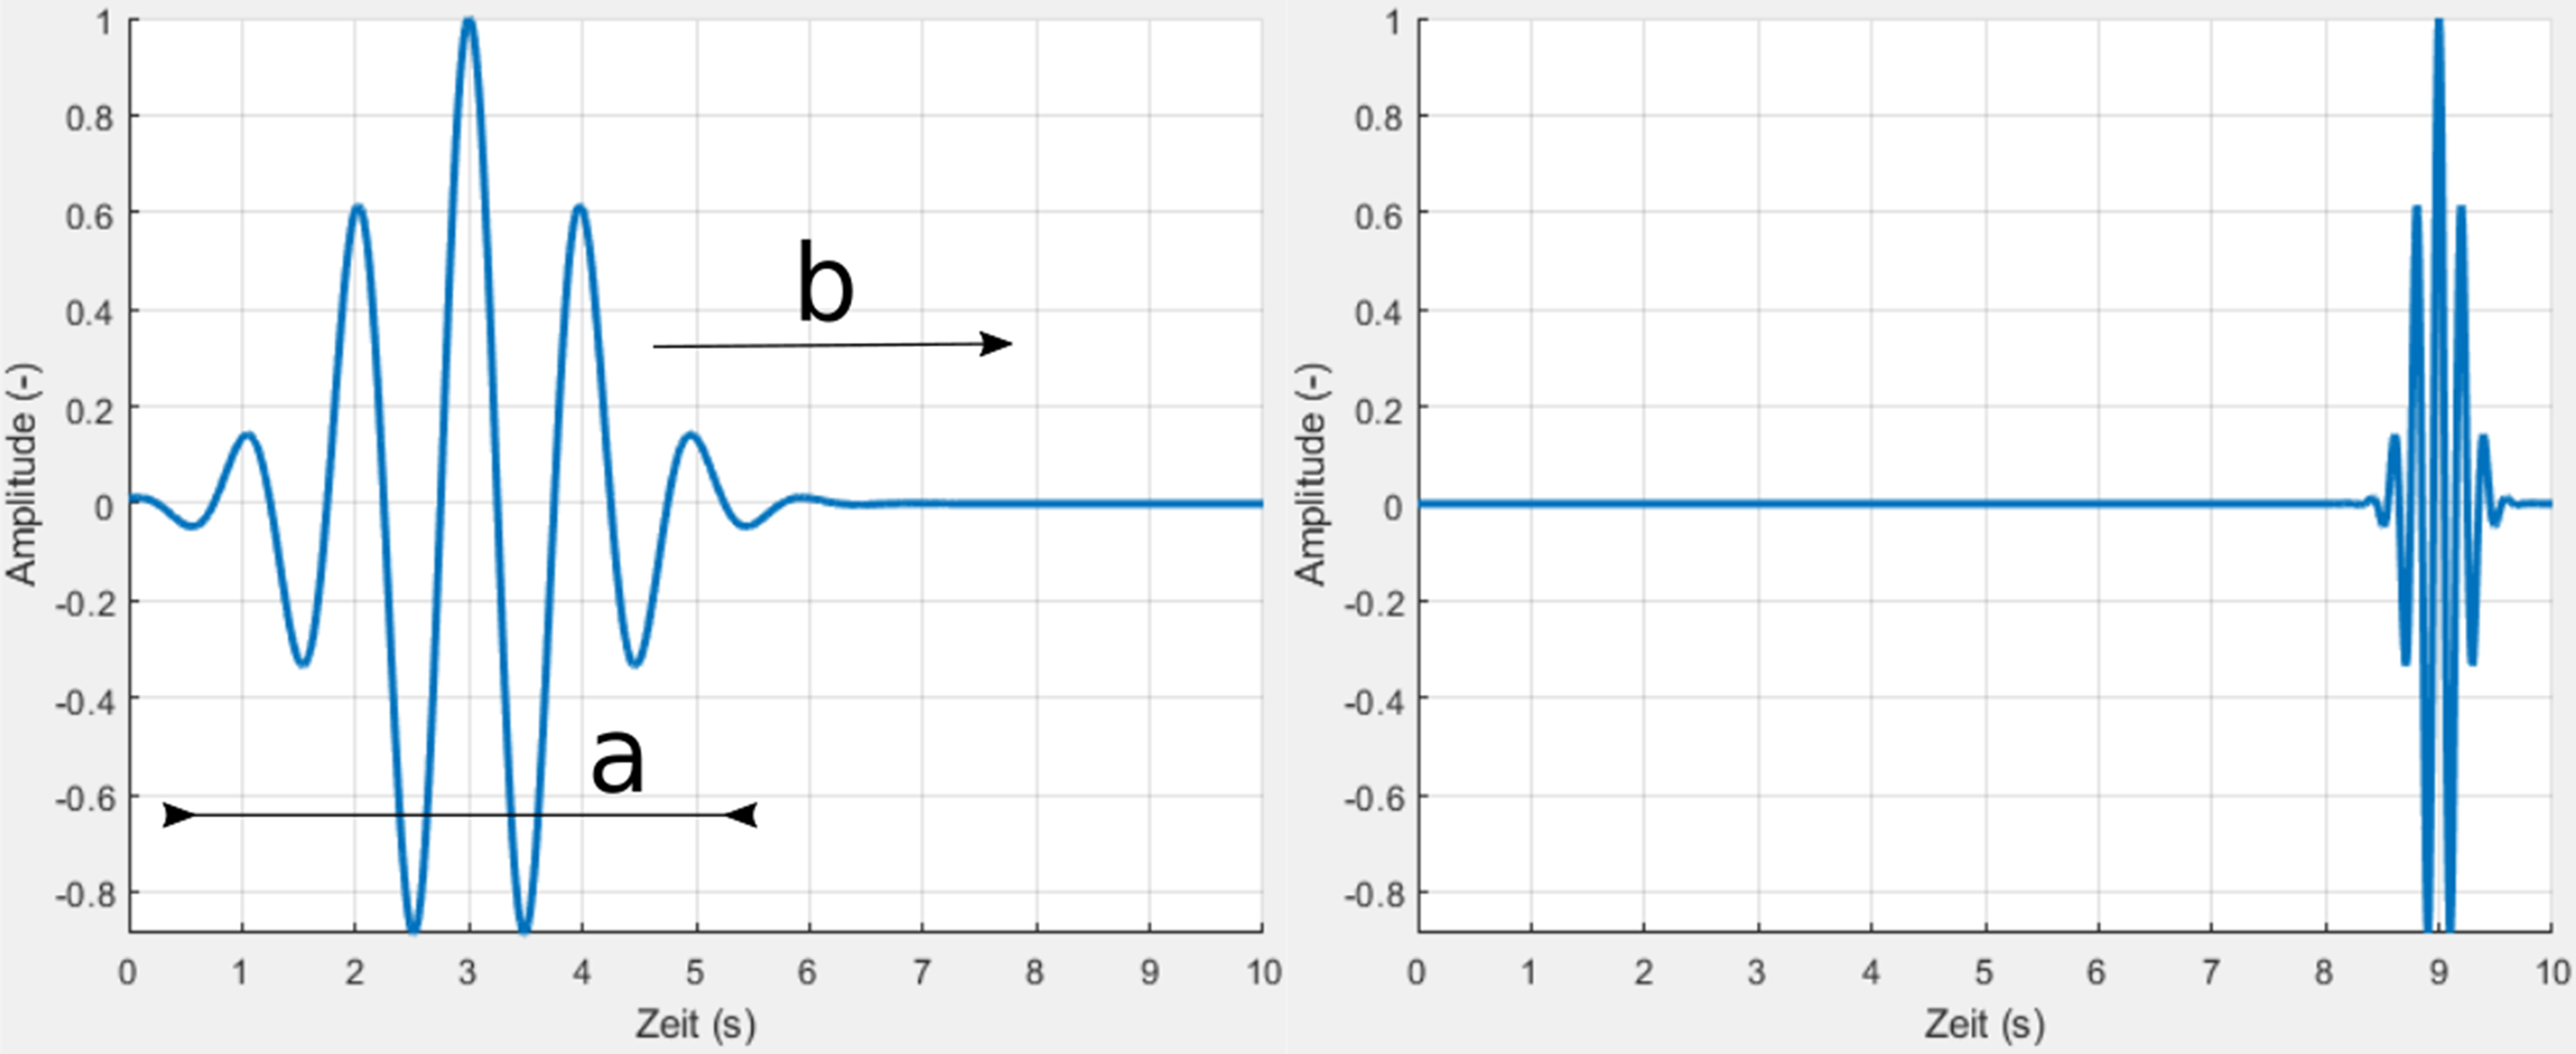
\includegraphics[width=0.75\textwidth]{papers/wavelets/images/5_WaveletKompUndShift.png}
	\caption{Darstellung der Wavelet Komprimierung a und der Verschiebung b}
	\label{wavelet:fig:5_WaveletKompUndShift}
\end{figure}

Hierbei handelt es sich um einen Kernpunkt der Anwendung der Wavelet Transformation, ihre grosse Stärke ist nämlich die zeitlich exakte Auflösung. Um der Wavelet Transformation die gleiche Maske wie der DFT zu geben, kann man
\begin{equation}
	W_{a,b}=\sum_{a=f_0}^{a_n}\sum_{b=0}^{b_m}\frac{1}{N(a)}\sum_{n=0}^{N-1} x(n)\cdot\psi\left(\frac{t-b}{a}\right)
	\label{wavelets:equation4}
\end{equation}
als Summenformel nachvollziehen. Die Formel deutet an, dass der Berechnungsaufwand deutlich ansteigen wird, sofern mit hoher Frequenz und Zeitauflösung gerechnet wird.

Die Relation zwischen der Auflösung von Frequenz und Zeit ist ein Kernthema in der Signalanalyse. Bei der DFT kann entweder die Zeit oder die Frequenz genau aufgelöst werden. Beides zusammen ist an sich nicht möglich,
weil bedingt durch die Unschärferelation sind Zeit- \& Frequenzauflösung ein komplementäres Paar, wodurch nicht beides gleichzeitig exakt bestimmbar ist. Anders ausgedrückt, die beiden Auflösungen bedingen eine gegensätzliche Periodenlänge. Ein schmales Fenster, welches die Periodenbreite bestimmt, ergibt eine hohe Zeit-, aber schlechte Frequenzauflösung. Ein breites Fenster führt demnach gerade zum Gegenteil.
Dieses konträre Verhalten kann relativ einfach mit folgender Überlegung nachvollzogen werden.
\begin{itemize}
\item Um eine Frequenzauflösung von 0.1 Herz zu erhalten, braucht es mit $f=1⁄T$ eine Zeitperiode von 10s, was einer sehr guten Frequenzauflösung entspricht, handkehrum bekommt man auch immer nur für die Periode von 10 Sekunden eine zeitliche Information. Wenn bei dieser Auflösung bestimmt werden soll ob es nach 1, 4 oder 10 Sekunden zum Event kam, ist das nicht bestimmbar.
\end{itemize}
 
Man kann mit gewissen Kniffen dem entgegen wirken. Beispielsweise mit Hilfe von Signalüberlappung oder Zero Padding.
\begin{itemize}
	\item Bei der Signalüberlappung wird das Auswertungsfenster mit einer Überdeckung verschoben. Dabei ist $2/3$ ein gängiger Wert für diese Überdeckung, es muss erwähnt sein, dass es dabei mehr um die Problematik des Informationsverlustes als um die bessere zeitliche Auflösung geht.
	\item Beim Zero Padding wird die Periodenbreite künstlich mit Nullen verbreitert. Man kann sich das mit einer Doppelfensterung vorstellen, das innere Fenster dient der hohen zeitlichen Auflösung und das äussere Fenster der besseren Frequenzauflösung und alles was zwischen dem inneren und äusseren Fenster liegt wird mit Nullen befüllt. Dadurch kann sowohl die Zeit als auch die Frequenzauflösung erhöht werden. Durch die künstliche Verbreiterung geht aber die Amplitudengenauigkeit verloren.
\end{itemize}
Die Unschärfeproblematik in (Abbildungen \ref{wavelet:fig:FFTAufloesung} und \ref{wavelet:fig:AufloesungZeitVsFrequenz}) bleibt aber bestehen.

\begin{figure}
	\centering
	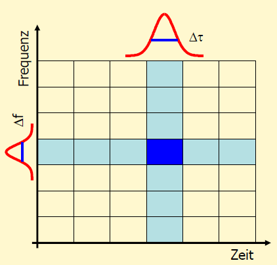
\includegraphics[width=0.3\textwidth]{papers/wavelets/images/6-1_FFTAufloesung.png}
	\caption{Schematische Darstellung der Unschärfeproblematik, entweder wird die Zeit oder die Frequenzgenauigkeit verfeinert (dargestellt anhand er beiden Achsrichtungen)}
	\label{wavelet:fig:FFTAufloesung}
\end{figure}

\begin{figure}
	\centering
	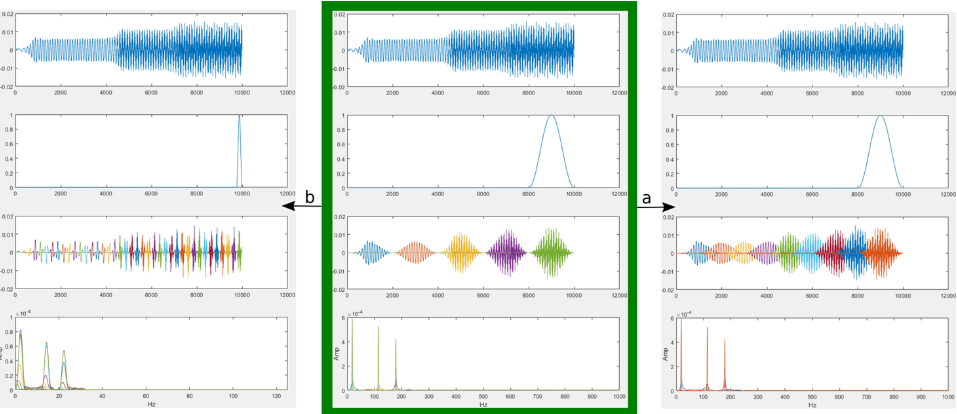
\includegraphics[width=\textwidth]{papers/wavelets/images/6-2_AufloesungZeitVsFrequenz.png}
	\caption{Unschärfeproblematik dargestellt an der FFT mit einem Hanning-Fenster. Im obersten Plot pro Gruppe ist jeweils das Zeitsignal das mit dem darunter liegenden Fenster verrechnet wird. Im untersten Plot der Gruppe ist der zugehörige Amplitudengang abgebildet. Mit grün hinterlegt ist die Ausgangsauswertung mit einer Fensterbreite von 1s, was einer Frequenzauflösung von 1Hz entspricht. Der Weg a beschreibt die Möglichkeit der Fensterüberlappung, die Fensterbreite bleibt dabei 1s. Der Weg b stellt die Auswertung mit einem schmaleren Fenster der breite $1/5$ s dar (5Hz Auflösung). Die zeitliche Auflösung kann dadurch deutlich verbessert werden. Am Amplitudengang ist aber die schlechtere Frequenzauflösung an den breiter werdenden Peaks zu erkennen.}
	\label{wavelet:fig:AufloesungZeitVsFrequenz}
\end{figure}

Das Wavelet hingegen besitzt die Eigenschaft, dass sowohl zeitlich als auch auf der Frequenz zugleich eine hohe Auflösung erzielt werden kann. Es besitzt sowohl in der Skalierung als auch in der Verschiebung einen freien Parameter. Wie bereits erwähnt geht das aber Hand in Hand mit einem hohen Berechnungsaufwand, sofern beides hoch aufgelöst werden soll. Ausserdem unterliegt das Wavelet durch seine endliche Energie Formulierung einer gewissen Verschmierung bei der Transformation ins Frequenzspektrum. Die Bandbreite im Amplitudengang ist wesentlich grösser als bei der FFT, weil Frequenzen nahe der zentralen Frequenz stärker betont werden. Die zeitliche Auflösung und die Detektion von zeitlichen Veränderungen durch das Wavelet ist hingegen fantastisch (schematisch in Abbildung \ref{wavelet:fig:CWTAufloesungRadix2} \& anschaulich in Abbildung \ref{wavelet:fig:ErsteAnwendung}).

\begin{figure}
	\centering
	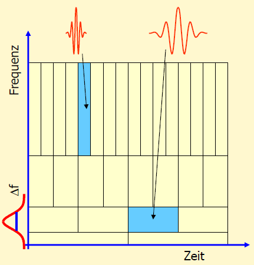
\includegraphics[width=0.3\textwidth]{papers/wavelets/images/6-3_CWTAufloesungRadix2.png}
	\caption{Schematische Darstellung der Auflösungsmöglichkeit bei der Wavelettransformation. Zeit und Frequenz können nach freiem belieben aufgelöst werden (separate Parameter), im der Darstellung verdeutlicht an einer Radix 2 Filterbank. Die Idee dahinter, das bei tiefen Frequenzen bedingt durch die Wellenlänge eine schlechtere Zeitauflösung genügt und erst bei kurzen Wellenlängen (hoher Frquenz) eine höhere zeitliche Auflösung benötigt wird.}
	\label{wavelet:fig:CWTAufloesungRadix2}
\end{figure}

Das Mutter-Wavelet $\psi\left(\frac{t-b}{a}\right)$ kann ganz verschiedene Funktionen besitzen, dargestellt in Abbildung \ref{wavelet:fig:MutterwavletTypen}, welche aber zwei Vorgaben einhalten müssen:

\begin{figure}
	\centering
	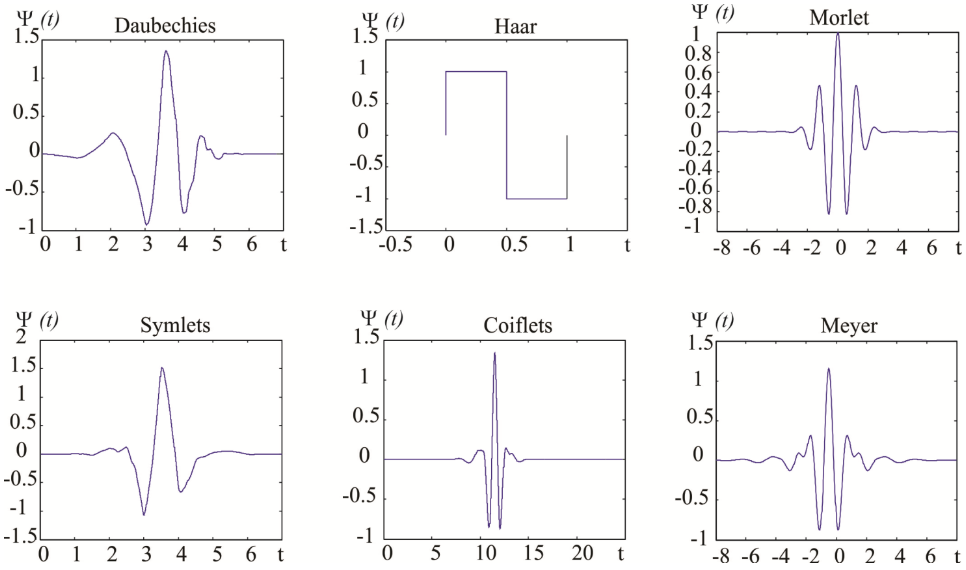
\includegraphics[width=0.75\textwidth]{papers/wavelets/images/6-4_MutterwavletTypen.png}
	\caption{Beispiele von verschiedenen Mutterwavelettypen.}
	\label{wavelet:fig:MutterwavletTypen}
\end{figure}

\begin{itemize}
	\item Der Mittelwert des Wavelet muss Null sein, ansonsten würde das Signal bei der Verrechnung durch das Wavelet gewichtet.
	\item Das Wavelet muss eine endliche Energie $||\psi||_2<\infty$ besitzen. Als Konsequenz aus der Cauchy-Schwarz-Ungleichung muss
	\begin{equation}
		\int_{-\infty}^{\infty} f(t)\cdot\psi\left(\frac{t-b}{a}\right) dt
		\label{wavelets:equation5}
	\end{equation}
	einen endlichen Wert besitzen. Im Gegensatz dazu hat beispielsweise ein reiner Sinus bei dieser Integration einen unendlichen Wert. In dieser Bedingung versteckt sich gerade auch noch eine weitere Eigenschaft welche die Wavelettransformation gegenüber der herkömmlichen Fourier-Transformation besitzt. Die Gewichtung wird vom Wavelet selbst und nicht über die Verrechnung mit einer Fensterfunktion getätigt.
\end{itemize}



%\subsection{De finibus bonorum et malorum
%\label{wavelets:subsection:finibus}}
%blabla \eqref{wavelets:equation1}.

%Et harum quidem rerum facilis est et expedita distinctio
%\ref{wavelets:section:teil2}.
%test
%\ref{wavelets:section:teil3}.



